\documentclass{beamer}
\usepackage{tikz,amsmath,hyperref,graphicx,stackrel,animate,media9}
\usetikzlibrary{positioning,shadows,arrows,shapes,calc}
\newcommand{\argmax}{\operatornamewithlimits{argmax}}
\newcommand{\argmin}{\operatornamewithlimits{argmin}}
\mode<presentation>{\usetheme{Frankfurt}}
\AtBeginSection[]
{
  \begin{frame}<beamer>
    \frametitle{Outline}
    \tableofcontents[currentsection,currentsubsection]
  \end{frame}
}
\title{Lecture 7: Frequency Response}
\author{Mark Hasegawa-Johnson}
\date{ECE 401: Signal and Image Analysis, Fall 2020}  
\begin{document}

% Title
\begin{frame}
  \maketitle
\end{frame}

% Title
\begin{frame}
  \tableofcontents
\end{frame}

%%%%%%%%%%%%%%%%%%%%%%%%%%%%%%%%%%%%%%%%%%%%
\section[Review]{Review: Convolution and Fourier Series}
\setcounter{subsection}{1}

\begin{frame}
  \frametitle{What is Signal Processing, Really?}

  \begin{itemize}
  \item When we process a signal, usually, we're trying to
    enhance the meaningful part, and reduce the noise.
  \item {\bf Spectrum} helps us  to understand which part is
    meaningful, and which part is noise.
  \item {\bf Convolution} (a.k.a. filtering) is the tool we use to
    perform the enhancement.
  \item {\bf Frequency Response} of a filter tells us exactly which
    frequencies it will enhance, and which it will reduce.
  \end{itemize}
\end{frame}

\begin{frame}
  \frametitle{Review: Convolution}
  \begin{itemize}
  \item A {\bf convolution} is exactly the same thing as a {\bf weighted local average}.
    We give it a special name, because we will use it very often.  It's defined as:
    \[
    y[n] = \sum_m g[m] f[n-m] = \sum_m g[n-m] f[m]
    \]
  \item 
    We use the symbol $\ast$ to mean ``convolution:''
    \[
    y[n]=g[n]\ast f[n] = \sum_m g[m] f[n-m] = \sum_m g[n-m] f[m]
    \]
  \end{itemize}
\end{frame}

\begin{frame}
  \frametitle{Review: Spectrum}

  The {\bf spectrum} of $x(t)$ is the set of frequencies, and their
  associated phasors,
  \[
  \mbox{Spectrum}\left( x(t) \right) =
  \left\{ (f_{-N},a_{-N}), \ldots, (f_0,a_0), \ldots, (f_N,a_N) \right\}
  \]
  such that
  \[
  x(t) = \sum_{k=-N}^N a_ke^{j2\pi f_kt}
  \]
\end{frame}

\begin{frame}
  \frametitle{Review: Fourier Series}

  One reason the spectrum is useful is that {\bf\em any} periodic
  signal can be written as a sum of cosines.  Fourier's theorem says that
  any $x(t)$ that is periodic, i.e.,
  \[
  x(t+T_0) = x(t)
  \]
  can be written as
  \[
  x(t) = \sum_{k=-\infty}^\infty X_k e^{j2\pi k F_0 t}
  \]
  which is a special case of the spectrum for periodic signals:
  $f_k=kF_0$, and $a_k=X_k$, and
  \[
  F_0 = \frac{1}{T_0}
  \]
\end{frame}

\begin{frame}
  \begin{itemize}
  \item {\bf Fourier Series Analysis}  (finding the spectrum, given the waveform):
    \[
    X_k = \frac{1}{T_0}\int_0^{T_0} x(t)e^{-j2\pi kt/T_0}dt
    \]
  \item {\bf Fourier Series Synthesis}  (finding the waveform, given the spectrum):
    \[
    x(t) = \sum_{k=-\infty}^\infty X_k e^{j2\pi kt/T_0}
    \]
  \item {\bf DFT Analysis}  (finding the spectrum, given the waveform):
    \[
    X[k] = \sum_{n=0}^{N-1} x[n]e^{-j2\pi kn/N}
    \]
  \item {\bf DFT Synthesis} (finding the waveform, given the spectrum):
    \[
    x[n] = \frac{1}{N}\sum_{k=0}^{N-1} X[k] e^{j2\pi kn/N}
    \]
  \end{itemize}
\end{frame}  

%%%%%%%%%%%%%%%%%%%%%%%%%%%%%%%%%%%%%%%%%%%%
\section[Frequency Response]{Frequency Response}
\setcounter{subsection}{1}

\begin{frame}
  \begin{block}{Frequency Response}
    The {\bf frequency response}, $G(\omega)$, of a filter $g[n]$, is
    its output in response to a pure tone, expressed as a function of
    the frequency of the tone.
  \end{block}
\end{frame}

\begin{frame}
  \frametitle{Calculating the Frequency Response}
  \begin{itemize}
  \item {\bf Output of the filter:}
    \begin{align*}
      y[n] &= g[n]\ast x[n]\\
      &= \sum_m g[m] x[n-m]
    \end{align*}
  \item {\bf in response to a pure tone:}
    \[
    x[n] = e^{j\omega n}
    \]
  \end{itemize}
\end{frame}

\begin{frame}
  \frametitle{Calculating the Frequency Response}

  \noindent{\bf Output of the filter in response  to a pure tone:}
  
  \begin{align*}
    y[n] &= \sum_m g[m] x[n-m]\\
    &= \sum_m g[n] e^{j\omega (n-m)}\\
    &= e^{j\omega n} \left(\sum_m g[m] e^{-j\omega m}\right)
  \end{align*}
  Notice that the part inside the parentheses is not a function of
  $n$.  It is not a function of $m$, because the $m$ gets summed over.
  It is only a function of $\omega$.  It is called the frequency
  response of the filter, $G(\omega)$.
\end{frame}

\begin{frame}
  \begin{block}{Frequency Response}
    When the input to a filter is a pure tone,
    \[
    x[n] =e^{j\omega n},
    \]
    then its output is the same pure tone, scaled and phase shifted by  a  complex number
    called the {\bf frequency response} $G(\omega)$:
    \[
    y[n] = G(\omega) e^{j\omega n}
    \]
    The frequency response is related to the impulse response as
    \[
    G(\omega) = \sum_m g[m]e^{-j\omega m}
    \]
  \end{block}
\end{frame}

%%%%%%%%%%%%%%%%%%%%%%%%%%%%%%%%%%%%%%%%%%%%
\section[Example]{Example: First Difference}
\setcounter{subsection}{1}

\begin{frame}
  \frametitle{Example: First Difference}

  \centerline{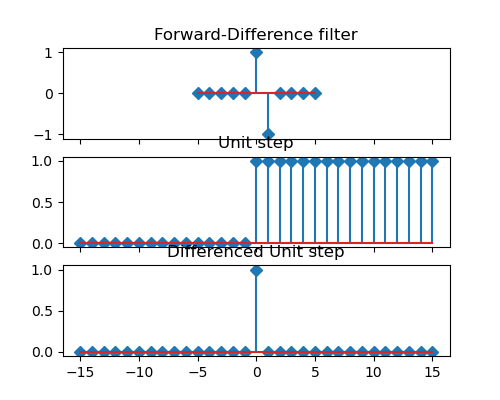
\includegraphics[height=1in]{../lec02/mp1fig5.png}}
  
  Remember that taking the difference between samples can be written as a convolution:
  \[ y[n] = x[n]-x[n-1]= g[n]\ast x[n],\]
  where
  \[
  g[n]=\begin{cases}1 & n=0\\-1&n=1\\0&\mbox{otherwise}\end{cases}
  \]
\end{frame}

\begin{frame}
  \frametitle{Example: First Difference}

  Suppose that the input is a pure tone:
  \[
  x[n] = e^{j\omega n}
  \]
  Then the output will be
  \begin{align*}
    y[n] &= x[n]-x[n-1]\\
    &= e^{j\omega n} -e^{j\omega (n-1)}\\
    &= G(\omega) e^{j\omega n},
  \end{align*}
  where
  \[
  G(\omega) = 1-e^{-j\omega}
  \]
\end{frame}

\begin{frame}
  \frametitle{First Difference Filter at $\omega=0$}
  \[
  G(\omega) = 1-e^{-j\omega}
  \]
  \begin{itemize}
  \item Frequency $\omega=0$ means the input is a constant value:
    \[
    x[n] = e^{j\omega n}\vert_{\omega=0} = 1
    \]
  \item At frequency $\omega=0$, the frequency response is zero!
    \[
    G(0) = 1-e^{0} = 0
    \]
  \item \ldots which totally makes sense, because if $x[n]=1$, then
    \[
    y[n]=x[n]-x[n-1] = 1-1 = 0
    \]
  \end{itemize}
\end{frame}

\begin{frame}
  \frametitle{First Difference Filter at $\omega=\pi$}
  \begin{itemize}
  \item Frequency $\omega=\pi$ means the input is $(-1)^n$:
    \[
    x[n] = e^{j\pi n} = (-1)^n= \begin{cases}
      1 & n~\mbox{is even}\\
      -1 & n~\mbox{is odd}
    \end{cases}
    \]
  \item At frequency $\omega=\pi$, the frequency response is two!
    \[
    G(\pi) = 1-e^{j\pi} = 1 - (-1)  = 2
    \]
  \item \ldots which totally makes sense, because if $x[n]=(-1)^n$, then
    \[
    y[n]=x[n]-x[n-1] = \begin{cases}
      1-(-1) = 2 & n~\mbox{is even}\\
      (-1)-1 = -2 & n~\mbox{is odd}
    \end{cases}
    \]
  \end{itemize}
\end{frame}

\begin{frame}
  \frametitle{First Difference Filter at $\omega=\frac{\pi}{2}$}
  Frequency $\omega=\frac{\pi}{2}$ means the input is $j^n$:
  \[
  x[n] = e^{j\frac{\pi n}{2}} = j^n= \begin{cases}
    1 & n\in\left\{0,4,8,12,\ldots\right\}\\
    j & n\in\left\{1,5,9,13,\ldots\right\}\\
    -1 & n\in\left\{2,6,10,14,\ldots\right\}\\
    -j & n\in\left\{3,7,11,15,\ldots\right\}\\
  \end{cases}
  \]
  The frequency response is:
  \[
  G\left(\frac{\pi}{2}\right) = 1-e^{j\frac{\pi}{2}} = 1 - j,
  \]
  so $y[n]$ is
  \[
  y[n] = (1-j) e^{j\frac{\pi n}{2}} = (1-j) j^n= \begin{cases}
    (1-j) & n\in\left\{0,4,8,12,\ldots\right\}\\
    (j+1) & n\in\left\{1,5,9,13,\ldots\right\}\\
    (-1+j) & n\in\left\{2,6,10,14,\ldots\right\}\\
    (-j-1) & n\in\left\{3,7,11,15,\ldots\right\}\\
  \end{cases}
  \]
\end{frame}

%%%%%%%%%%%%%%%%%%%%%%%%%%%%%%%%%%%%%%%%%%%%
\section[Superposition]{Superposition and the Frequency Response}
\setcounter{subsection}{1}

\begin{frame}
  \begin{block}{Superposition and the Frequency Response}
    The frequency response obeys the principle of {\bf superposition}, meaning that
    if the input is the sum of two pure tones:
    \[
    x[n] = e^{j\omega_1 n} + e^{j\omega_2 n},
    \]
    then the output is the sum of the same two tones, each scaled by
    the corresponding frequency response:
    \[
    y[n] = G(\omega_1)e^{j\omega_1 n}+G(\omega_2)e^{j\omega_2 n}
    \]
  \end{block}
\end{frame}

\begin{frame}
  \frametitle{Response to a Cosine}
  There are no  complex exponentials in the real world.  Instead, we'd like to know
  the output in response to a cosine input.  Fortunately, a cosine
  is the sum of two complex exponentials:
  \[
  x[n] = \cos(\omega n) = \frac{1}{2}e^{j\omega n}+\frac{1}{2}e^{-j\omega n},
  \]
  therefore,
  \[
  y[n] = \frac{G(\omega)}{2}e^{j\omega n}+\frac{G(-\omega)}{2}e^{-j\omega n}
  \]
\end{frame}


\begin{frame}
  \frametitle{Response to a Cosine}
  What is $G(-\omega)$?  Remember the definition:
  \[
  G(\omega) = \sum_m g[m] e^{-j\omega m}
  \]
  Replacing every $\omega$ with a  $-\omega$ gives:
  \[
  G(-\omega) = \sum_m g[m] e^{j\omega m}.
  \]
  Notice that $g[m]$ is real-valued, so the only complex number on the RHS  is $e^{j\omega m}$.  But
  \[
  e^{j\omega m}=\left(e^{-j\omega m}\right)^*
  \]
  so
  \[
  G(-\omega) = G^*(\omega)
  \]
\end{frame}

\begin{frame}
  \begin{block}{Response to a Cosine}
    \begin{align*}
      y[n] &= \frac{G(\omega)}{2}e^{j\omega n}+\frac{G^*(\omega)}{2}e^{-j\omega n}\\
      &= \frac{|G(\omega)|}{2}e^{j\angle G(\omega)}e^{j\omega n} + 
      \frac{|G(\omega)|}{2}e^{-j\angle G(\omega)}e^{-j\omega n}\\
      &= \frac{|G(\omega)|}{2}e^{j\left(\omega n+\angle G(\omega)\right)} +
      \frac{|G(\omega)|}{2}e^{-j\left(\omega n+\angle G(\omega)\right)}\\
      &= |G(\omega)|\cos\left(\omega n+\angle G(\omega)\right)
    \end{align*}
  \end{block}
  \begin{block}{Magnitude and Phase Responses}
    \begin{itemize}
    \item The {\bf Magnitude Response} $|G(\omega)|$ tells you by how
      much a pure tone at $\omega$ will be scaled.
    \item The {\bf Phase Response} $\angle G(\omega)$ tells you by how much
      a pure tone at $\omega$ will be advanced in phase.
    \end{itemize}
  \end{block}
\end{frame}

%%%%%%%%%%%%%%%%%%%%%%%%%%%%%%%%%%%%%%%%%%%%
\section[Example]{Example: First Difference}
\setcounter{subsection}{1}

\begin{frame}
  \frametitle{Example: First Difference}

  Remember that the first difference, $y[n]=x[n]-x[n-1]$, is supposed
  to sort of approximate a derivative operator:
  \[
  y(t) \approx \frac{d}{dt} x(t)
  \]
  If the input is a cosine, what is the output?
  \[
  \frac{d}{dt} \cos\left(\omega t\right) = -\omega \sin\left(\omega t\right)
  = \omega \cos\left(\omega t+\frac{\pi}{2}\right)
  \]
  Does the first-difference operator behave the same way (multiply by
  a magnitude of $|G(\omega)|=\omega$, phase shift by $+\frac{\pi}{2}$
  radians so that cosine turns into negative sine)?
\end{frame}

\begin{frame}
  \frametitle{Example: First Difference}

  Freqeuncy response of the first difference filter is
  \[
  G(\omega) = 1-e^{-j\omega}
  \]
  Let's try to convert it to polar form, so we can find its magnitude and phase:
  \begin{align*}
    G(\omega) &= e^{-j\frac{\omega}{2}} \left(e^{j\frac{\omega}{2}}-e^{-j\frac{\omega}{2}}\right)\\
    &= e^{-j\frac{\omega}{2}} \left(2j\sin\left(\frac{\omega}{2}\right)\right)\\
    &= \left(2\sin\left(\frac{\omega}{2}\right)\right)\left(e^{j\left(\frac{\pi-\omega}{2}\right)}\right)
  \end{align*}
  So the magnitude and phase response are:
  \begin{align*}
    |G(\omega)| &= 2\sin\left(\frac{\omega}{2}\right)\\
    \angle G(\omega) &= \frac{\pi-\omega}{2}
  \end{align*}
\end{frame}

\begin{frame}
  \frametitle{First Difference: Magnitude Response}
  Taking the derivative of a cosine scales it by $\omega$.  The first-difference
  filter scales it by $|G(\omega)|=2\sin(\omega/2)$, which is almost the same, but not quite:
  \centerline{\includegraphics[height=2in]{exp/firstdiff_magnitude.png}}
\end{frame}

\begin{frame}
  \frametitle{First Difference: Phase Response}

  Taking the derivative of a cosine shifts it, in phase, by
  $+\frac{\pi}{2}$ radians, so that the cosine turns into a negative
  sine.  The first-difference filter shifts it by $\angle
  G(\omega)=\frac{\pi-\omega}{2}$, which is almost the same, but not
  quite.
  \centerline{\includegraphics[height=2in]{exp/firstdiff_phase.png}}
\end{frame}

\begin{frame}
  \frametitle{First Difference: All Together}
  Putting it all together, if the input is $x[n]=\cos(\omega n)$, the output is
  \[
  y[n]=|G(\omega)|\cos\left(\omega n+\angle G(\omega)\right)
  =2\sin\left(\frac{\omega}{2}\right)\cos\left(\omega n+\frac{\pi-\omega}{2}\right)
  \]
  \begin{itemize}
  \item At frequency $\omega=0$, the phase shift is exactly $\frac{\pi}{2}$,
    so the output is turned from cosine into -sine (but with an amplitude of 0!)
  \item At frequency $\omega=\pi$, the phase shift is 0!  So the output
    is just a cosine at twice the amplitude.
  \item In between, $0<\omega <\pi$,
    \begin{itemize}
    \item The amplitude gradually increases, while
    \item the phase gradually shifts, from a -sine function back to a cosine function.
    \end{itemize}
  \end{itemize}
\end{frame}

\begin{frame}
  \frametitle{First Difference: All Together}
  Putting it all together, if the input is $x[n]=\cos(\omega n)$, the output is
  \[
  y[n]=|G(\omega)|\cos\left(\omega n+\angle G(\omega)\right)
  =2\sin\left(\frac{\omega}{2}\right)\cos\left(\omega n+\frac{\pi-\omega}{2}\right)
  \]
  \centerline{\animategraphics[loop,controls,height=1.5in]{15}{exp/firstdiff_tonesweep}{0}{149}}
\end{frame}

%%%%%%%%%%%%%%%%%%%%%%%%%%%%%%%%%%%%%%%%%%%%
\section[Linearity]{Linearity}
\setcounter{subsection}{1}

\begin{frame}
  \begin{block}{Linearity}
    Filters are linear: if you scale the input, the output also scales.  Thus if
    \[
    x[n] = Ae^{j\omega_1 n} + Be^{j\omega_2 n},
    \]
    then the output is the sum of the same two tones, each scaled by
    the corresponding frequency response:
    \[
    y[n] = G(\omega_1)Ae^{j\omega_1 n}+G(\omega_2)Be^{j\omega_2 n}
    \]
  \end{block}
\end{frame}

\begin{frame}
  \frametitle{Response to a Cosine}
  Linearity applies to complex numbers, not just  real numbers!
  So if
  \[
  x[n] = A\cos(\omega n+\theta) = \frac{A}{2}e^{j(\omega n+\theta)}+\frac{A}{2}e^{-j(\omega n+\theta)},
  \]
  then
  \begin{align*}
    y[n] &= \frac{AG(\omega)}{2}e^{j(\omega n+\theta)}+\frac{AG^*(\omega)}{2}e^{-j(\omega n+\theta)}\\
    &= \frac{A|G(\omega)|}{2}e^{j(\omega n+\theta+\angle G(\omega))}+\frac{A|G(\omega)|}{2}e^{-j(\omega n+\theta+\angle G(\omega))}\\
    &= A|G(\omega)|\cos\left(\omega n+\theta+\angle G(\omega)\right)
  \end{align*}
\end{frame}

%%%%%%%%%%%%%%%%%%%%%%%%%%%%%%%%%%%%%%%%%%%%
\section[Summary]{Summary}
\setcounter{subsection}{1}

\begin{frame}
  \frametitle{Summary}
  \begin{itemize}
  \item {\bf Tones in $\rightarrow$ Tones out}
    \begin{align*}
      x[n]=e^{j\omega n} &\rightarrow y[n]=G(\omega)e^{j\omega n}\\
      x[n]=\cos\left(\omega n\right)
      &\rightarrow y[n]=|G(\omega)|\cos\left(\omega n+\angle G(\omega)\right)\\
      x[n]=A\cos\left(\omega n+\theta\right)
      &\rightarrow y[n]=A|G(\omega)|\cos\left(\omega n+\theta+\angle G(\omega)\right)
    \end{align*}
  \item where the {\bf Frequency Response} is given by
    \[
    G(\omega) = \sum_m g[m]e^{-j\omega m}
    \]
  \end{itemize}
\end{frame}  
        
\end{document}
